\documentclass[12pt,openright,oneside,a4paper,brazil,article]{abntex2}

\usepackage[brazil]{babel}
\usepackage[utf8]{inputenc}
\usepackage[T1]{fontenc}
\usepackage{enumerate} 
\usepackage{amssymb}
\usepackage{bbm}
\usepackage{tikz}
\usepackage{graphicx}
\usepackage{subcaption}
\usepackage{wrapfig}
\usepackage[framemethod=PStricks]{mdframed}
\usepackage{colortbl}
\usepackage{xcolor}
\usepackage{courier}
\usepackage{multicol}
\usepackage[onelanguage,portuguese,ruled,noend]{algorithm2e}
\usepackage[hmargin=2cm,vmargin=2cm,bmargin=2cm]{geometry}
\usepackage{lplfitch}
\usepackage{amsmath}
\usepackage{amsfonts}
\usepackage{amssymb}
\usetikzlibrary{automata,positioning}

\newcommand{\algofont}{\small}
\renewcommand\AlCapFnt{\algofont}
\SetAlgoRefName{}
\SetAlgoCaptionSeparator{}

\setlist[itemize]{itemsep=0mm}
\setlist[enumerate]{itemsep=0mm}

\everymath{\displaystyle}

\begin{document}
  \textual
  \SingleSpacing

  \begin{wrapfigure}{l}{1.3cm}
    
\includegraphics[scale=0.18]{uva.png}
  \end{wrapfigure}

  \noindent \textbf{Universidade Estadual Vale do Acaraú - UVA} \\
  \noindent \textbf{Curso:} Ciência da Computação \\
  \noindent \textbf{Disciplina:} Introdução a Ciências da Computação\\
  \noindent \textbf{Professor:} Eder Jacques Porfirio Farias \\

  \begin{center}
    \textbf{ICC - AP3} \\
    \textbf{WebPong(BETA v0.1.0)} 
  \end{center}

% Nas listas em grupo basta descomentar as linhas 57 e 58

  \noindent Aluno(a): Ilder Rafael Damasceno Ponte \textbf{Programador} \\
  \noindent Aluno(a): Rafael Cordeiro Araujo Lima \textbf{Revisor de Codigo}\\
  \noindent Aluno(a): Luis Fernando Paiva de Souza \textbf{Testar o jogo e reportar bugs/Apresentação}\\
  \noindent Aluno(a): Caio Monte Mendes \textbf{Testar o jogo e reportar bugs/Apresentação}\\
  
  \begin{abstract}
  O trabalho se basia na criação de uma versão online multiplyer do jogo Pong,
  onde dois jogadoes em computadoes distntos jogam em uma mesma sala. Para criar 
  o jogo se usarão as tecnologias: \textbf{ReactJS, NodeJS, WebSocket}. Sendo a 
  aplicação dividida entre "server" e "front". Os dados serão processados no "server"
  e o front será responsavél por mostrar o jogo na tela. Ademais o jogo deve conter
  um sistema de chat e salas.
  \end{abstract}
  
  \begin{enumerate}
    \item \textbf{Introdução}
    \paragraph*{O programa utiliza o \textbf{ReactJS} para conseguir manusear componentes e valores de uma melhor forma
    de inicio vamo explicar a função basica de cada script do projeto, sendo que cada um desses é um componente.}
    \begin{itemize}
      \item \textbf{index.js:} Este é o responsável por ligar a aplicação a pagina \textbf{index.js}
      presente no diretório \textit{./public}, o que torna a aplicação visivel a todos.
      \item \textbf{app.js:} Este é responsável pela união dos componentes \textbf{pong.js} e \textbf{styleGlobal.js}.
      \item \textbf{styleGlobal.js:} Este é responsável pelo estilo da aplicação como um todo. Para gerenciar o estilo 
      é utilizada a "biblioteca" \textbf{styled-components}.[Ele também passa algumas propriedades("props") para o \textbf{pong.js}]
      \item \textbf{pong.js:} Este é responsável por juntar e organizar todos os componentes para o funcionamento da
      aplicação. Nele também são definidas as propriedades("props") utilizadas nos componentes, elas são obtidas com o 
      \textbf{useContext} que importa o "contexto" do \textit{script} \textbf{GameContext.js}.
      \item \textbf{roomList.js:} Este é responsável por listar as salas disponives e os botoes relacionados a salas
      \item \textbf{playerList.js:} Este é responsável por listar os \textit{players} na tela.
      \item \textbf{chat.js:} Este é responsável por gerenciar o chat e menssagens.
      \item \textbf{game.js} Este é responsável por desenhar o jogo na tela, para isso usa a "biblioteca" \textbf{react-svg-draw}.
      \item \textbf{gameContext.js:} Este é responsavél por gerenciar a comunicação com o \textbf{server.js} utilizando o \textbf{Socket}. 
      \item \textbf{server.js:} Esté  é responsável por gerenciar as informações gerais d aplicação, como as salas, os players, e o jogo.
    \end{itemize}
    \item \textbf{Execução} \\
    \paragraph*{Para executar basta seguir os seguintes passos:}
    \begin{itemize}
      \item Abra dois terminais(cmd, powershell, bash, etc.), um na pasta \textit{./gameserver} e outro na pasta \textit{./gamefront}
      
      \item Depois digite os seguintes comandos\\\\
      npm install
      \\
      npm start

      \item Depois basta abrir no endereço \textit{http://localhost:3000}[Na versão final o jogo funcionará em LAN, mas nesse caso basta apenas abrir em duas guias diferentes]
    \end{itemize}
    \item \textbf{Problemas Conhecidos}
    \begin{itemize}
      \item \textbf{Demora na desconacção:} Quando a pessoa recarrega a pagina varias vezes pode acontecer de o "player" anterior que 
      era a propria pessoa não se disconect, isso acontece devido a um atraso por "afogamento"(varias chamadas feitas de uma só vez) no \textbf{Socket} devido a varias requisisções, 
      mas não afeta em nada o desenpenho da apliação.
      \item \textbf{Falta das barras:} As barras ainda não foram adicionadas no jogo devido a necessidade de se ter que fazer pesquisas para ver
      como funcionará a colisão, mas nada muito dificil.
      \item \textbf{"Match is null":} Esse erro pode aparecer devido a um bug envolvendo "afogamento" no \textbf{Socket}, mas é raro.
    \end{itemize} 
    
    \textbf{"FLUXOGRAMA" e IMAGENS:}
    \begin{center}
      \begin{wrapfigure}{l}{1.3cm}
        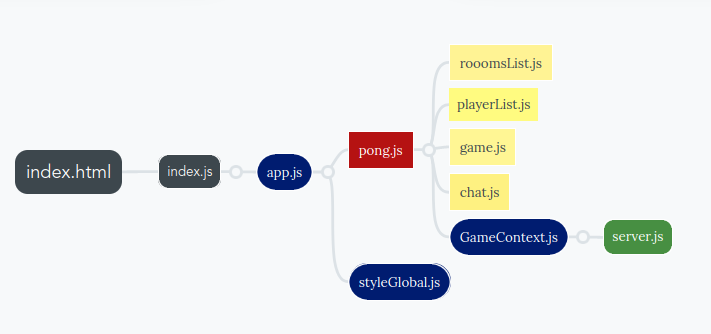
\includegraphics[scale=1]{fluxograma.png}
      \end{wrapfigure}  
    \end{center}

    \begin{center}
      \begin{wrapfigure}{l}{1.3cm}
        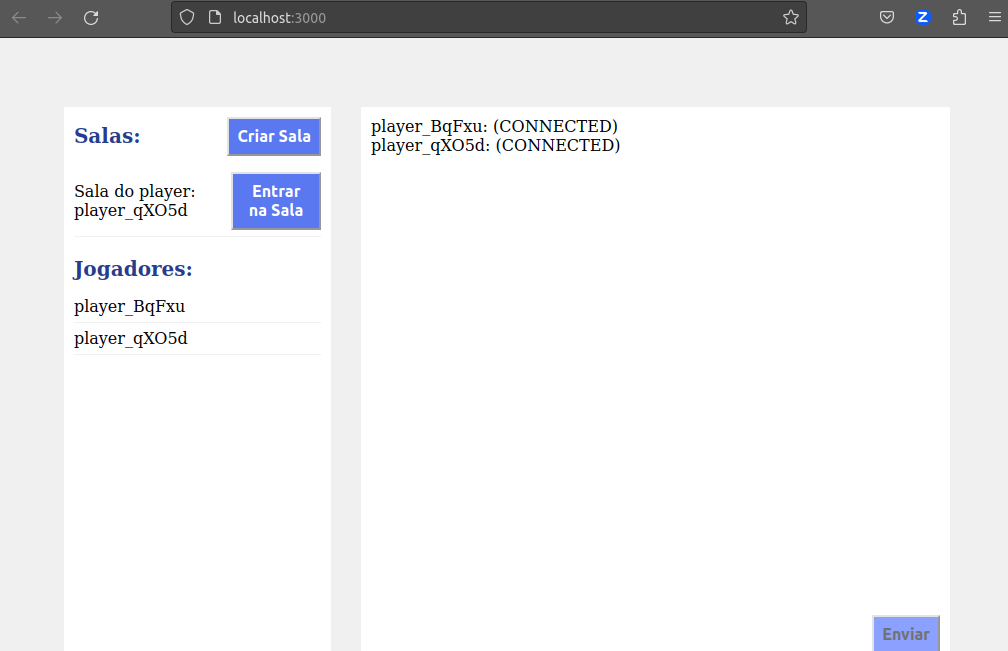
\includegraphics[scale=1]{gamescreen1.png}
      \end{wrapfigure}  
    \end{center}
    

    \begin{center}
      \begin{wrapfigure}{l}{1.3cm}
        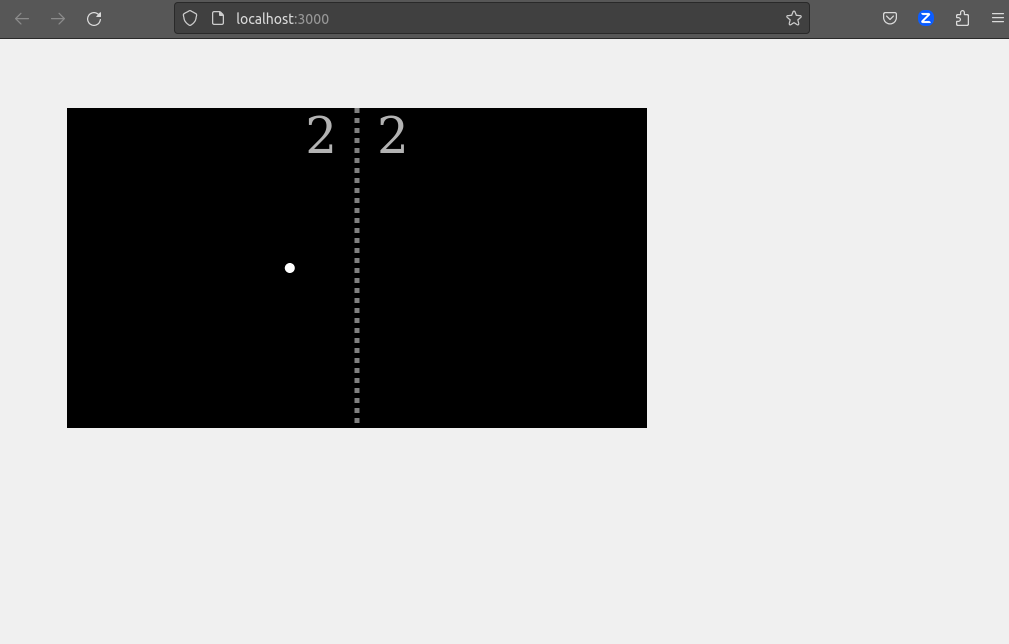
\includegraphics[scale=1]{gamescreen2.png}
      \end{wrapfigure}  
    \end{center}
  \end{enumerate}
\end{document}